\documentclass[article,type=msc,colorback,12pt,accentcolor=tud7b]{tudthesis}
\usepackage{ngerman}
\usepackage[english]{babel}
\usepackage{cite}
\usepackage{hyperref}
\graphicspath{ {images/A/} {images/B/} {images/C/} }

\hypersetup{
    colorlinks,
    citecolor=blue,
    filecolor=blue,
    linkcolor=blue,
    urlcolor=blue
}


\newcommand{\getmydate}{%
  \ifcase\month%
    \or Januar\or Februar\or M\"arz%
    \or April\or Mai\or Juni\or Juli%
    \or August\or September\or Oktober%
    \or November\or Dezember%
  \fi\ \number\year%
}

\begin{document}
  \thesistitle{Feedback Driven Development of Cloud Applications} 
  %\linebreak[1]Corporate-Design f"ur {\LaTeX}!}%
    {Feedback Driven Development of Cloud Applications}
  \author{Harini Gunabalan}
  \birthplace{}
  \referee{Prof. Dr.-Ing. Mira Mezini}{Dr. Guido Salvaneschi, Dr. Gerald Junkermann, Aryan Dadashi}
  \department{Department of Computer Science}
  \group{Software Technology Group}
  \dateofexam{31 May 2015}{31 May 2015}
  \tuprints{12345}{1234}
  \makethesistitle
  \affidavit{Harini Gunabalan}


\begin{abstract}
\begin{large} 
	
\par Over the last few years, the Cloud Computing Paradigm has gained a lot of importance in both the Academia and the Industry. The cloud has not only changed the IT Landscape from the user's perspective but has also changed how the Developers develop applications on the cloud. The increasing adoption of the DevOps approach has led to the removal of the boundaries between the development and the operations. 



\par Among the the three levels of the Cloud Computing: Infrastructure-as-a-Service (IaaS), Platform-as-a-Service(PaaS) and Software-as-a-Service(SaaS), Software Developers are mainly concerned with the PaaS which allows them to focus on the Application Development. Leveraging the fact that the Application is hosted on the cloud, there are additional metrics regarding the application available to Developers in different Log formats. There are also Cloud Monitoring Tools which consolidates these logs with a huge volume of data representing the run-time metrics etc. of the cloud applications. Though monitoring of the cloud applications has been done by many tools, most of the developers do not go through the cumbersome error/warning log data.These log data are not visually made available to the developers in their Development Environment. By providing this information, developers can have an overview of the Application Performance at real time, and can capture issues that occur at scale which normally could not be captured by Profilers. This could also help us to reduce the developer-operator gap providing an improved DevOps experience. 

\par This Thesis work aims in addressing this issue. The focus is mainly to map the run-time metrics to the source code artifacts, thereby helping the developers link the Run time metrics to the source code. Mapping will involve log data aggregation, code analysis techniques etc.

	
\end{large}
\end{abstract}  

\clearpage

%=====INDEX================================================================================
\setlength{ \parskip }{1em}
\index{key}
\tableofcontents 
\cleardoublepage 

\listoffigures
\clearpage
\appendix
\cleardoublepage 

% abstract, acknowledgements, contents
 \section{Introduction}
	
	Cloud Computing is one of the fields in Computer Science that has gained rapid growth and importance in the recent years. The fact that the servers are remote hosted rather than local servers has led to innumerable small scale businesses. Start-ups no longer require high infrastructure, instead they just need to pay for the amount of resources that they actually use (pay-per-use). This also significantly reduces the initial monetary setup costs for such start-ups. There has been extensive research in Cloud Computing areas such as auto-scaling of resources at the infrastructure level, monitoring of metrics at both the application and infrastructure level. However, there is not much research done in how these monitored metrics are utilized by the Cloud Application Developers. Making the run-time metrics visibly effective for the developers in their Development Environment is the issue this thesis is aiming to solve.
	\par This chapter is structured into four sections. The first section provides the motivation of this thesis work. The second section gives an insight into the problem statement which this Thesis work aims to solve. The third section details the contribution of the work and the fourth section provides how the following chapters of the Thesis are structured.
	
	\subsection{Motivation}
	
	Software Engineering Practice in the industry has faced a phenomenal change since the advent of Cloud Computing. This is mainly due to the flexibility and the dynamic scaling up and scaling down of the infrastructure as required by the current workload. This proves not only to be elastic but cost-effective as well. It is quite obvious that this elasticity is achieved by the continuous monitoring of several metrics that indicate the demand at the moment, and provisioning the necessary resources to meet the monitored demand. Distributed, scalable enterprise-wide applications also mandate the monitoring of metrics for reasoning the effectiveness of the applications by engineers and business analysts \cite{leitner2012application}.
	
	\par The metrics that are being monitored vary widely. For instance, the metrics such as memory consumption, CPU utilization, Network bandwidth utilization could be considered to be at the Infrastructure level, whereas some other metrics such as Response times of methods/procedures, the number of users accessing the application, maximum number of users who can use the application simultaneously, etc. could be considered to be at the application level. Sometimes, the application level metrics could depend on the primitive metrics at the infrastructure level and vice-versa.
	
	\par As Cloud Application Development has becoming more common, the run time monitoring metrics of these applications are available through several Application Performance Monitoring (APM) tools such as Amazon Cloudwatch, New Relic, etc. But, they do not provide any valuable and visible feedback to the developers, and hence most of the cloud developers do not use it. However, this run-time monitoring data could be used to provide useful analytic information such as performance hotspots that is taking a lot of execution time, and predictive information such as methods or loops that may become critical, even before the deployment. This type of analytic and predictive feedback should be provided to the developers in their IDEs which otherwise may not be explored by the developers. This technique of utilizing the monitoring data is known Feedback driven development. Feedback Driven Development that provides visual tools to the cloud developers is the focus of this thesis research.	
	
	\subsection{Problem Statement}	
	
The Cloud computing paradigms are classified into three service models which forms a stack as shown in Figure 1. 

 \begin{figure}
 \begin{center}
  \makebox[\textwidth]{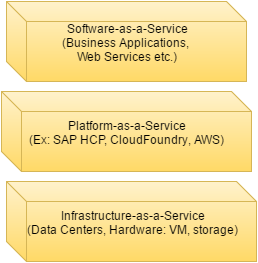
\includegraphics[scale=0.7]{A1}}
\end{center}
\caption{Cloud Computing Stack}
\end{figure}

%\begin{itemize}
%	
%	\item Infrastructure-as-a-Service
%	
%	\item Platform-as-a-Service
%	
%	\item Software-as-a-Service  
%% add the stack image 	
%\end{itemize}
	
\cite{bruneo2015framework} defines a framework that collects data as defined by a 3-D cloud monitoring model. From the software engineering perspective, it is important to note how Cloud Computing impacts the development practices. Based on the research conducted, there are two important research issues \cite{cito2014making}. 

\begin{itemize}

	
	\item Impact of DevOps on Cloud Application Developers:	
	The Cloud Developers are forced to look into the huge log data of the cloud applications. Development and Operations are brought much closer than the traditional software methods. Sometimes the same person acts as both the developer and the operator. 
	
	\item Data and Tools utilized by Cloud Developers:
	The data produced by the logs include Business Metrics, System-level Data etc. Sometimes the implementation changes may even have monetary consequences in the cloud, nevertheless most of the developers do not pay attention to this aspect. Hence it can be argued that once these operational metrics are brought closer to the Cloud Developers Environment, they would be able to pay closer attention to this information thereby achieving cost-effective applications.
	
\end{itemize}

Considering these issues, it is certainly important how we are going to leverage these Cloud monitoring Logs to make a useful impact for the Cloud Developers. 
 
 	\subsubsection{Continuous Delivery in Cloud Development}
 	As we compare the software development on-premise with that of the Cloud, there has been a huge change in every software release. Deployment cycles has been reduced from months to days and sometimes even within a few hours the next version is released. This process is often referred to Continuous Delivery(CD) in the Cloud Computing terms. Most companies make use of this Continous Delivery to rollout new features and evaluate their new ideas in a controlled manner \cite{kohavi2007practical}. CD has become a huge success and companies such as Google,Facebook etc. adopt CD of varying degrees for some of their services. When a feature is delayed for the current roll-out, it gets delayed by months when the traditional software development life-cycle is used. The feature needs to be delayed until the next release. Whereas in this CD approach the next release could be in the same day or in the same week, leading to small changes of production code. This also leads to a state called "perpetual development" where the code is always under continuous development and there is no stable release version for a particular product.  	\par Owing to this new release paradigm, there are a lot of extra information generated. The live performance of the application, click-streams from the User Interface of application, error and warning logs, infrastructure related data etc. are produced. There are a lot of existing APM Tools that collect this data and generate information out of it, however, how this information could be made effective to the software developers in their daily routine is a topic that is not discussed very often. 
 	
 	\subsubsection{Monitoring Metrics: Scalability and Availability of the Application}
 	
	Some of the monitoring metrics collected include the CPU usage, response time of the request, number of instances the application is hosted on, no. of requests each instance serves during a particular time period, error logs of the request etc. While these metrics focus mainly at the Infrastructure level, the logs instrumented into the application are also collected. We use these metrics to focus on two main challenges of cloud computing: Scalability and Availability of the Cloud applications.
	
	\par Scalability is the ability to increase or decrease the resources of an instance or the number of instances so that the changing demand of the incoming requests can be met. The platform related log data are collected for both Horizontal scaling (increasing the number of instances) and Vertical scaling(increasing the resources of each instance).
	
	\par Availability is one of the major goals of Cloud Computing. It means that the Cloud Services need to be available and accessible at anytime from anywhere. For business to happen continuously, it is necessary for the services to be highly available. The definition of availability is specified by the different Cloud vendors in their SLAs. For example, Google Search is known for its high availability.	
	
	\subsubsection{Incorporating the collected Feedback in the Development Environment}	
	
	Using the collected metrics, in this thesis, we aim to provide an efficient feedback to the Cloud Developers. The collected feedback is integrated into the Development Environment (IDEs) so that developers are able to utilize the feedback to make their applications better scalable and highly available.	
	
	
	\subsection{Contribution}
	
	\subsection{Structure of the Thesis}

	\par This thesis is structured in six chapters. Chapter 1 provides a short introduction into the topic and describes the goals of the thesis. Chapter 2 includes more background information and presents the state of the art of the important topics of this thesis: Cloud Application Performance Monitoring(AMP) tools, Feedback Driven Development(FDD) in general, and how FDD could be useful for Cloud Application Developers. The third Chapter describes an overview of the high-level System Design and the design decisions made in this research work. The fourth chapter explains the system on a lower fine-grained level. Interesting Implementation details are also provided here. Chapter 5 shows the various case studies, evaluates the developed system and illustrates its usage as well as possible applications. Finally, Chapter six provides the conclusion of the thesis and outlines the future work ideas.

% Example of Footnote    
%     \textbf{Alle Vordefinierten Texte sind, wie verbindlich vorgeschrieben, in der hessischen Amtssprache
%    gehalten\footnote{Deutschland hat (noch) keine Amtssprache.}.}

	\cleardoublepage

 \section{State of the Art}
 	
	This chapter presents the state of art of the topics relevant for this thesis. In the first section, we explain what is Cloud Monitoring. The second section briefs about Auto-scalers and third section provides a background on Data Modeling. The fourth section describes about mining source code changes to identify performance regressions and the final section details about Feedback Driven Development and the types of FDD. 
	
	\subsection{Cloud Monitoring}
 	
 	As Cloud Computing is gaining popularity, the need for Cloud monitoring is becoming increasingly important to  both the Cloud Providers and the Cloud Consumers. At the Cloud Provider side, Cloud Monitoring is the key principle behind which the actual controlling of hardware takes place. It enables them to scale the infrastructure, if necessary. On the Cloud Consumer side, Cloud Monitoring enables to check the Availability, QoS etc. of the applications. The consumers can verify any SLA violations by comparing the Key Performance Indicators(KPI) parameters provided by Cloud Monitoring.
 	
 	\cite{aceto2013cloud} explains in detail about the need for Cloud Monitoring: the basic concepts involved, the properties which needs to be maintained, and finally also lists down the open issues with respect to Cloud monitoring. These are summarized in Figure 2.
	
	There are several Cloud monitoring platforms and services such as CloudWatch \cite{cloudwatchdev} \cite{cloudwatch}, AzureWatch \cite{azurewatch} , NewRelic \cite{newrelic} etc. Table 1 provides a list of Cloud Monitoring platforms and services. Amazon CloudWatch provides users the monitored information for 2 weeks. Users are allowed to plot these information, set thresholds, alerts etc and these alerts can be used to perform any substantial action such as sending an Email or even in AutoScaling \cite{aas}. AutoScaling is explored in detail in the next section. 
	
\begin{table}[h!]
  \centering
  \caption{Cloud Monitoring Platforms and Services }
  \label{tab:Table1}
  \begin{tabular}{l|l}
  \hline
  \textbf{Cloud Monitoring Platforms}  & \textbf{Cloud Monitoring Services} \\
    \hline
    CloudWatch \cite{cloudwatchdev} \cite{cloudwatch} & New Relic \cite{newrelic} \\    
    Nimsoft \cite{nimsoft} & Cloudyn \cite{cloudyn} \\        
    AzureWatch \cite{azurewatch} & Up.time \cite{uptime} \\        
    Nagios \cite{nagios} & CloudSleuth \cite{cloudsleuth} \\
    Nimbus \cite{nimbus} & Cloudstone \cite{cloudstone} \\ 
    GroundWork \cite{groundwork} & Boundary \cite{boundary} \\
    LogicMonitor \cite{logicmonitor} & Cloudfloor \cite{cloudfloor} \\ 
    CloudKick \cite{cloudkick} & CloudClimate \cite{cloudclimate} \\    
    Monitis \cite{monitis} & CloudHarmony \cite{cloudharmony} \\
    \hline
    
  \end{tabular}
\end{table}
	
	Some other Cloud Monitoring Platforms such as Nimsoft Monitoring Solution \cite{nimsoft} provides a unified monitoring dashboard to view infrastructures provided by Salesforce, Rackspace, Google or Amazon. Nagios \cite{nagios} is a popular open source Cloud Monitoring platform which provides monitoring of virtual machines and storage (Amazon EC2 and S3). It also supports OpenStack \cite{openstack}, an open Source Cloud IaaS. New Relic \cite{newrelic} is a web-based Monitoring service that helps to monitor the application infrastructure and performance, adhering to timeliness, resilience, availability and accuracy.
	
	While all of the above Cloud Monitoring platforms and services are great, most of them do not consider multiple layers or real-time data. Some of them consider multiple layers whereas do not take into account the real-time data, and some consider real-time data but do not consider the multiple cloud layers \cite{marquezan20143}. \cite{bruneo2015framework} proposes a 3D-Cloud Monitoring framework called the Ceiloesper framework, which combines monitoring in multiple layers with real time data and it also performs the data analysis for multiple management actions. It is based on the Complex event processing (CEP) and uses the Esper CEP Engine.
 		
%	\subsection{Logging}
%		
%		As depicted in \cite{jiang2009understanding} , it is clear that Auto Generated issues are resolved much faster than human generated issues. Auto generated issues are those that have attached symptoms and system logs as event messages, whereas Human generated issues are those reported by the users usually through email tickets/phone calls. This further justifies the use and necessity of logging. \cite{jiang2009understanding} also lists down the challenges of using the logging information.
%		
%		The Log Data collected to generate the feedback is discussed here. Among the two types of data: Monitoring Data and Production data as detailed in \cite{cito2015runtime} we focus on the Monitoring data. This category of data is further classified as Load Data (incoming requests, server utilization, number of instances), Performance data (Response times, hotspots), cost data and User Behavior Data (Click Streams). This data is mostly collected by existing APM Tools.
%		
%		\cite{yuan2012conservative} answers the question of where to add logs proactively that could help minimize the effort of failure diagnosis. ERRLOG, a tool that identifies in which location log needs to be added is developed. Errlog makes use of code analysis techniques to achieve this. iTrack, a framework for monitoring user activities and correlating them with system data is done to detect service outages as in \cite{mann2011correlating}. 
%			
%	\subsubsection{Logging Tools and Metrics}	
%
%		\subsubsection{Log Structure}	
%		
%		\subsubsection{Performance related Logging}
%		\cite{nagaraj2012structured} explains a tool known as DISTALYZER that analyses the system logs to identify the performance issues. This tool analyses logs from large scale distributed systems and compares a set of baseline logs with an acceptable performance with another set of logs with unacceptable performance. DISTALYZER uses machine learning techniques which first creates a set of features(event/state variables) for the logs. Further Predictive and Descriptive Modeling are performed on these variables to provide the developers the root cause of the issue.
%
%		\subsubsection{Click Stream Logging}
	

\begin{figure}
 \begin{center}
  \makebox[\textwidth]{\includegraphics[width=\textwidth]{B5}}
\end{center}
\caption{Cloud Monitoring \cite{aceto2013cloud}}
\end{figure}	
	
	\subsection{Auto-scaling}	
	
	Scaling of Cloud Infrastructure means changing the current infrastructure. It could be of two types: Horizontal and Vertical Scaling. Horizontal Scaling is a methodology of adding/removing machines whereas vertical scaling is increasing/decreasing the resources such as CPU/Memory/Disk to existing machines.
	
	The Metrics monitoring and Data Collection has a huge importance with respect to Auto-scaling. Auto-scaling or automatic scaling is a process where the Cloud Platform adapts itself by increasing or shutting down the number of instances on which the application is currently deployed depending on the current load. For enterprises running their own infrastructure shutting down servers that are not being utilized could save electricity costs, whereas for enterprises running their applications on Cloud, auto-scaling could lead to saving costs due to the pay-per-use model of the Cloud. Auto-scaling also improves the efficieny of applications. In the scenario mentioned in \cite{bunch2012pluggable}, auto-scaling improves the instance utilization of the open source AppScale PaaS by 91\% and it also brings down the average time taken to serve the requests. Auto-scalers can be broadly classified as the following: 
	
	\begin{itemize}
	
	\item{Reactive Auto-scaling: }Auto-scaling as provided by most of the cloud providers such as Amazon Web Services, Microsoft Azure, and IBM Bluemix etc are reactive. This means based on monitoring the relevant metrics, whenever a certain metric increases or decreases beyond a particular predefined threshold, additional instances are added or removed. This method which is more of a rule-based mechanism is a reactive auto-scaling method. This is easier to be implemented as it involves monitoring metrics, and framing rules and policies for scaling. While this method serves in most scenarios, the question arises whether it is capable to handle bursty traffic.
	
	In \cite{seelam2015polyglot} the rule based reactive autoscaler of IBM's Bluemix PaaS, Polyglot application, is described. Polyglot autoscaler allows application developers to set thresholds based on which instances need to be added (scale-out) or removed (scale-in). These threshold values could be parameters such as CPU Utilization, memory and heap usage. The architecture of the Polyglot autoscaler can be found in Figure 3. It consists of the four components: Agents which collect the performance information, a monitoring service which continuously monitors the health of the cloud application, a scaling service which makes the decision of whether scaling needs to be performed or not, and a Persistence service to keep track of the enactment points (points where the application is scaled in time).  

\item{Predictive Auto-scaling: }Predictive auto-scaling comes very handy to handle bursty workloads. By analyzing the historic time series data, it may be possible to predict the workload at a future time, thereby enabling predictive auto-scaling. The effectiveness of this method depends on the efficiency of the workload prediction.

\cite{biswas2015predictive} introduces a predictive auto scaling technique that uses a Machine Learning engine to make predictions based on a deadline driven algorithm for predicting the future state of the system. \cite{Scryer1} and \cite{Scryer2} describes a predictive auto-scaling tool, Scyer, used by Netflix to provision the correct number of Amazon Web Services \cite{aws} instances. This is different from the Amazon AutoScaling(AAS) \cite{aas}, which is a reactive one. Scryer's prediction engine is able to provision the resources based on two prediction algorithms to predict the workload. The prediction algorithms implemented are augmented linear regression based algorithm and Fast Fourier Transformation based algorithm.

\item{Hybrid Auto-scaling: } Hybrid Auto-scaling is a combination of both the Reactive and Predictive approaches. As mentioned in \cite{Scryer1}, Scryer tool works in co-ordination with the AAS for more efficient auto scaling. \cite{moore2013coordinated} describes the architecture and implementation of Platform Insights, which is another hybrid auto-scaler that employs a reactive rule-based and a predictive model-based approach in a coordinated manner.
\end{itemize}
Auto-scalers face the following problems as listed in \cite{lorido2014review}:
\begin{description}
	\item[Under Provisioning:] The application is hosted on lesser infrastructure than that is necessary to process all the incoming requests. Due to Service-level-agreements (SLA's), it takes a while for it to reach up to the required amount of infrastructure. This could also lead to SLA violations.
	
	\item[Over Provisioning:] There is no SLA violations in this scenario. However the actual amount of resources is greater than the required amount of resources and hence the customer could be paying extra cost that his actual usage.
	
	\item[Oscillation:]
		When there is an oscillation between Under Provisioning and Over Provisioning it causes an undesirable and unstable state. 
\end{description}

In order to solve this, auto scaling needs to focus on the MAPE Loop\cite{lorido2014review}: Monitor, Analyze, Plan and Execute. The necessary monitoring metrics are collected and analyzed to decide on the type of autoscaling: reactive/predictive/hybrid. The planning phase is done on how to actually perform the scaling: Horizontal/Vertical. Finally the actual scaling is performed based on SLA.

 \begin{figure}
 \begin{center}
  \makebox[\textwidth]{\includegraphics{B4}}
\end{center}
\caption{Architecture of polyglot autoscaler \cite{seelam2015polyglot}}
\end{figure}

	\subsection{Data Modeling}
	
	Correlation and Covariance are two important concepts in statistics. Both indicate how closely two variables are related. For instance if variable X increases, will variable Y increase or decrease or does not depend on X. In addition to this, correlation helps us to understand to what extent the two variables change with respect to each other. 

\par
Correlation could be either positive or negative. If the variable Y increases proportionately when variable X in increased by a unit, it is known as positive correlation. On the other hand if the variable Y decreases proportionately when variable X is increased it is a negative correlation. This can be explained graphically as shown in Figure 4. If all the points are centered around the straight line: Y = X, then X and Y are said to be positively correlated. Whereas if all the points are centered around a line Y = -X, then X and Y are said to be inversely correlated. If all the points are scattered throughout then there is no correlation between variables X and Y. Figure 4 depicts positive, negative and no correlation.

\par
According to statistics, if $X_i$ and $Y_i$ are sample data for the two variable under consideration then correlation can be calculated as \cite{correlation}: $$ Correlation, r_{xy} = S_{xy} / S_x S_y $$ where $S_x$ = sample standard deviation of variable X, $S_y$ = sample standard deviation of variable Y and $S_{xy}$ is the sample covariance of the variables X and Y. The correlation coefficient values $r_{xy}$ ranges between -1 and 1. If the value is positive, then there is a positive correlation and if the value is negative, then there is a negative correlation. If the value is 0 then there is no correlation. Also, the closer the values are to +1 or -1, the stronger is the correlation, positive or negative respectively.
\par
So far we considered only a single input variable, X and a single output variable, Y. However in reality most of the systems tend to be multiple-input multiple-output (MIMO) systems rather than the single-input single-output (SISO) system. The data that we deal in real world does not contain just 2 attributes. Most of the real world scenario involves a minimum of 5 to 6 dimensions and depending on the applications this may go as high as 20 or even more. Hence we explore further into multivariate correlation models: State Space Models, and Polynomial Models.

 \begin{figure}
 \begin{center}
  \makebox[\textwidth]{\includegraphics[width=\textwidth]{B7}}
\end{center}
\caption{Positive, Negative and no Correlation between X and Y }
\end{figure}

\subsubsection{State Space Models}

State space model represents a system by a set of First order differential equations, and state variables. Mathematically it can be described that the output Y(t) of a system at time, t can be predicted for any time t > $t_0$,  where $t_0$ is an initial time, and provided that we know the input and output of the system at time $t_0$ and a minimum set of variable $x_i(t)$ where i = 1 to n. In this case, n is the order of the state space model \cite{rowell2002state}. 

Figure 5 shows a system described by a state space model. The vector $u_1$, $u_2$, $u_3$,...,$u_i$ are the inputs while the output vector is $y_1$, $y_2$,....,$y_k$. By knowing the inputs and outputs at time $t_0$ the state variables: $x_1$, $x_2$, $x_3$,....,$x_n$ are first measured. Then it becomes possible to predict the output at any future time, t by knowing the inputs at that time and the measured state variables.

 \begin{figure}
 \begin{center}
  \makebox[\textwidth]{\includegraphics[scale=0.7]{B6}}
\end{center}
\caption{System represented by State Space Model}
\end{figure}

In state space modeling, the time derivative of the state variables are represented as a function of the state variable, and inputs, $dx/dt = f(x,u,t)$. Considering a Linear Time Invariant(LTI) systems, we have the state equation \cite{rowell2002state}: $$ dx/dt = Ax + Bu $$ where A and B are matrices with constant coefficients that weight the system's state variable and inputs respectively. Similarly the output equation can be written as \cite{rowell2002state}: $$ y = Cx + Du $$ where C and D are matrices with constant coefficients that weight the system's state variables and inputs respectively. There are several physical systems where the D matrix is found to be a null matrix thereby reducing the output equation to $ y = Cx $, where the output depends on a weighted combination of the state variables.

\subsubsection{Polynomial Models}
	
	Some physical systems do not always adhere to linear equations. Hence to model these type of systems we consider polynomials. Additionally there could be systems which depends on the previous values of the inputs, previous values of the outputs as well. Based on these we have the following four polynomial models \cite{ljung1998system}:
	
	\begin{enumerate}
		\item{ARX Model:} The ARX model to evaluate the output is based on Auto-regression(the past output values) and inputs. Auto regressive model is a model whose current output depends on the past values. The generic notion to denote auto-regressive model of order p, AR(p) for a variable X is: $$ X_t = c + \sum_{i=1}^{p} \rho_i X_{t-i} + e(t) $$ where c and $ \rho_i $ are constants and e(t) is the noise \cite{arma}. Considering auto regression and the inputs the ARX model can be mathematically described as: $$ A(z) y(t) = B(z) u(t-n) + e(t) $$ where y(t) is the output, u(t) is the input, and e(t) is the noise/error measured in the output. A(z) and B(z) are polynomials of the specified order with respect to the backward shift operator $Z^{-1}$. For example, $Z^{-n}  u(k)$ = $u(k-n)$ \cite{arx}.
		
	\item{ARMAX Model:} Unlike the ARX model, in ARMAX the stochastic dynamics are considered. Therefore this model handles a system where there is a domination of noise. ARMAX models are better for systems with more disturbances. In generaö, the moving average model of order q, MA(q) is represented in the below notation: $$ X_t =  e(t) + \sum_{i=1}^{q} \theta_i e(t-i) $$ where $ \theta_i $ are constants and e(t) and e(t-i) are the noise/errors \cite{arma}. The notation for the Auto-regressive moving average(ARMA) model is as below: $$ X_t = c + e(t) + \sum_{i=1}^{p} \rho_i X_{t-i} + \sum_{i=1}^{q} \theta_i e(t-i) $$ This model includes both AR(p) and MA(q) models. Based on these we have the following mathematical equation to for the ARMAX model: $$ A(z) y(t) = B(z) u(t-n) + c(Z) e(t) $$ where, y(t) is the output, u(t)is the input, and e(t) is the noise. A(z), B(z) and C(z) are polynomials of specified orders with respect to the backward shift operator $Z^{-1}$ \cite{armax}. 
	
	\item{Output-Error Model:} 
		The notation for the Output Error model is as below: $$ y(t) = [B(z)/F(z)] u(t-n) + e(t) $$ where, y(t) is the output, u(t)is the input, and e(t) is the noise. B(z) and F(z) are polynomials of specified orders with respect to the backward shift operator $Z^{-1}$ \cite{oe}.
	
	\item{Box-Jenkins Model:} 	
		 The notation for the Box Jenkins model is as below: $$ y(t) = [B(z)/F(z)] u(t-n) + [C(Z)/D(Z)] e(t) $$ where, y(t) is the output, u(t)is the input, and e(t) is the noise. B(z), F(z), C(z) and D(z) are polynomials of specified orders with respect to the backward shift operator $Z^{-1}$ \cite{bj}.
		 
	\end{enumerate}
	
	\subsection{Performance Analysis using Source Code History in Evolving Software}
	
	 Software evolution is defined as the change of characteristics of a software with time. Continuous Delivery has led to continuously evolving software. This means frequent code changes are prevalent and this naturally causes performance regressions. Performance of a software is quite important and hence valuating performance regressions during code changes becomes a necessity. Performance regression can be defined as a state when the application under consideration behaves worse in a new code deployment compared to its previous deployment. In this section we look into two source code mining tools: PerfImpact \cite{luomining} and LITO \cite{sandoval2016learning}.
	 \begin{enumerate}
	 \item{PerfImpact:} 
	 PerfImapct identifies the Performance Regressions and recommends potential code changes that has led to the performance degradation. PerfImpact achieves this as a two step-process: 
	 
	 \begin{itemize}
\item{\textbf{Identification of Inputs which cause the Performance Regression:}} 
\newline
PerfImpact defines a "Fitness Function" that determines the inputs which cause the delay in execution of a newer code deployment V\textsubscript{i+1} compared to its previous deployment V\textsubscript{i}. The fitness function makes use of Genetic Algorithms to achieve this. 
 
\item {\textbf{Mining execution traces to identify code changes that lead to Performance Regressions:}} 
\newline
PerfImpact also has a "Mining Function", which identifies those methods which take a longer execution time in V\textsubscript{i+1} compared to V\textsubscript{i}. These methods are tagged as Potentially problematic methods. Between the two deployments there could be several code changes/commits. Each code change is ranked based on the number of potentially problematic methods involved. The code changes with higher number of problematic methods are ranked higher and considered as the possible root cause for the performance regression. 	 
	 
	 \end{itemize}
	
PerfImpact was evaluated on two open source web applications: JPetStore\cite{Jpetstore} and Agilefant\cite{Agilefant}. Figure 6 shows the source code changes in two versions of Agilefant. The evaluation shows that the inputs which cause Performance regressions are identified efficiently. PerfImpact also lists the potentially harmful code changes which could be used further in Code Inspectors and Root Cause Analysis.

 \begin{figure}
 \begin{center}
  \makebox[\textwidth]{\includegraphics[width=\textwidth]{B1}}
  \makebox[\textwidth]{\includegraphics[width=\textwidth]{B2}}
\end{center}
\caption{Source Code Changes of two versions in Agilefant \cite{luomining}}
\end{figure}

 \begin{figure}
 \begin{center}
  \makebox[\textwidth]{\includegraphics{B3}}
\end{center}
\caption{Code Changes that caused maximum Performance Variations \cite{sandoval2016learning}}
\end{figure}

\item{LITO, a Horizontal Profiling technique:} 
LITO is a cost model to determine if a code commit has caused performance regressions based on sampling the execution of versions. This approach resolves the following research questions (RQs) as below:

\begin{itemize}

\item RQ-1: Is there a set of specific methods which will cause performance variations when the source code of these methods are modified? According to \cite{sandoval2016learning}, this is not really true. This is in contrast to PerfImpact. This approach was tested on 17 open source projects and the results showed that the methods, which cause performance variations before, not necessarily contributed to the performance variations in the newer versions.

\item RQ-2  What are the recurring code changes which affects the performance of an evolving software? The major code changes the caused performance variations are method call addition, method call deletion, method call swap, Complete Method call change, and Loop Addition  as compared to the other code changes listed in Figure 7 \cite{sandoval2016learning}.

\end{itemize}
\end{enumerate}	

	\subsection{Feedback Driven Development } 		
	
	 By analyzing any Cloud Application's logs, we can get hold of a huge amount of information. This can be broadly classified into: Application Level Logs and Infrastructure Level Logs. This data could be made useful to both the Developers and Operators. Infrastructure Logs provides details such as number of instances, the memory, CPU, Disk utilization of each instance, which instance serves a particular request etc. By making this kind of data visible to the developers, they can tweak the application development process, as they have access to the cloud internals. At the same time, the Cloud operators also benefit with the relevant business metrics to manage the instances more efficiently. 
	
	\par Collecting these run-time data, aggregating them into useful feedback, and feeding them back into the Development process of an application could create a useful impact in the future deployment of the application. This process is known as Feedback Driven Development(FDD). FDD can be classified into 2 types: Analytic FDD and Predictive FDD \cite{cito2015runtime}.
	
	\begin{itemize}
	\item{Analytic Feedback Driven Development: }
		Analytic FDD is the run time data from the previous deployments, which is brought directly into the developer environment. It provides a mapping between the log data collected and the source code artifacts. This helps the developers to understand how the run-time metrics directly impact the source code. Based on this developers can alter and optimize the code based on the real time user behavior. In practice, Analytic FDD deals with visualizing the run time operations data and how it is being mapped to the code artifacts. 
		
	\item{Predictive Feedback Driven Development: }
	Predictive FDD is one step ahead compared to the Analytic FDD. It utilizes the run-time feedback to warn the developers about the current code changes even before the updated source code is deployed. Predictive FDD is combined with static code analysis to give better predictions regarding a code change. 
	\end{itemize}
	
 \cleardoublepage
 \section{System Design}	
 
	In this chapter, the high level architectural design of the thesis work is explained. We look into the design decisions such as the choice of the metrics to be collected, the modeling methods and how the feedback is visualized in a productive manner to the developers.
 
\subsection{System Architecture Overview} 

	The architectural overview of the system is depicted in Figure C1. Initially,  a sample application for demo purpose is considered. This application is deployed in the cloud systems and monitored continuously. The data collected during this monitoring is extracted into a clean format to be used for the Modeling.
	
	\includegraphics[scale=0.7]{C1} 
	
The MATLAB System Identification Toolbox is used to model the data obtained. Using the model, we estimate the expected performance of the sample application. If a deviation occurs from this estimation then the root cause of the issue is analyzed. This is done by investigating the code changes such as code commits. Finally, the source code artifacts that is related to the anomaly is identified and visualized in the developer's IDE. Owing to the increased use of Continuous Delivery and DevOps approach, providing immediate run time production scenario to the Development 

\subsection{Monitoring Metrics} 

The deployed cloud app is monitored continuously to collect the various dimensions. In this thesis work, we focus on the following metrics:

 
 \subsection{System Architecture Details}
 	The overall system design is split into two phases as shown in the figure C2. The first phase explains the Modeling details and the second phase focuses on how the model is evaluated to identify the root cause that needs to be visualized as a feedback to the developers.
 	
\includegraphics[scale=0.6]{C2} 	
 	
 	A sample application is deployed into the Cloud. This application should be available for monitoring the parameters.
 	
 	\subsection{Phase 1: Modeling}
 	
 		\subsection{Phase 2: Evaluation of the Model}

 \cleardoublepage
 \section{System Implementation}
 \subsection{System Implementation}

 \cleardoublepage	  
 \section{Evaluation and Results}	  
 \subsection{Evaluation}
 
 \cleardoublepage
 \section{Conclusion and Future Work}	  
 \subsection{Conclusion and Future Work}

\clearpage
	  
%=====BIBLIOGRAPHY================================================================================
\bibliographystyle{ieeetr}
\bibliography{LatexRefThesis}	  

\end{document}
